\protect\hyperlink{main-nav}{≡} \protect\hyperlink{close-nav}{×}

\hypertarget{section-3.6-average-value-area-and-volume}{%
\section{Section 3.6: Average Value, Area, and
Volume}\label{section-3.6-average-value-area-and-volume}}

\hypertarget{average-value}{%
\subsection{Average Value}\label{average-value}}

We know the average of \textbackslash{}(n\textbackslash{}) numbers
\textbackslash{}(a\_1, a\_2, \textbackslash{}dots ,
a\_n\textbackslash{}) is their sum divided by
\textbackslash{}(n\textbackslash{}). But what if we need to find the
average temperature over a day's time -- there are too many possible
temperatures to add them up! This is a job for the definite integral.

To view this video please enable JavaScript, and consider upgrading to a
web browser that \href{http://videojs.com/html5-video-support/}{supports
HTML5 video}

\hypertarget{average-value-1}{%
\paragraph{Average Value}\label{average-value-1}}

The average value of a function \textbackslash{}(f(x)\textbackslash{})
on the interval \textbackslash{}({[}a, b{]}\textbackslash{}) is given by
\textbackslash{}{[}
\textbackslash{}frac\{1\}\{b-a\}\textbackslash{}int\_a\^{}bf(x)\textbackslash{},
dx. \textbackslash{}{]}

The average value of a positive \textbackslash{}(f\textbackslash{}) has
a nice geometric interpretation. Imagine that the area under
\textbackslash{}(f\textbackslash{}) (graph (a) below) is a liquid that
can ``leak'' through the graph to form a rectangle with the same area
(graph (b) below).

If the height of the rectangle is \textbackslash{}(H\textbackslash{}),
then the area of the rectangle is \textbackslash{}(
H\textbackslash{}cdot (b-a) \textbackslash{}). We know the area of the
rectangle is the same as the area under
\textbackslash{}(f\textbackslash{}) so \textbackslash{}(
H\textbackslash{}cdot (b-a) = \textbackslash{}int\_a\^{}b
f(x)\textbackslash{}, dx \textbackslash{}). Then \textbackslash{}{[} H =
\textbackslash{}frac\{1\}\{b-a\}\textbackslash{}int\_a\^{}b
f(x)\textbackslash{}, dx, \textbackslash{}{]} the average value of
\textbackslash{}(f\textbackslash{}) on
\textbackslash{}({[}a,b{]}\textbackslash{}).

The average value of a positive function
\textbackslash{}(f\textbackslash{}) is the height
\textbackslash{}(H\textbackslash{}) of the rectangle whose area is the
same as the area under \textbackslash{}(f\textbackslash{}).

\hypertarget{example-1}{%
\paragraph{Example 1}\label{example-1}}

During a 9 hour work day, the production rate at time
\textbackslash{}(t\textbackslash{}) hours after the start of the shift
was given by the function \textbackslash{}(
r(t)=5+\textbackslash{}sqrt\{t\} \textbackslash{}) cars per hour. Find
the average hourly production rate.

The average hourly production is \textbackslash{}(
\textbackslash{}frac\{1\}\{9-0\}\textbackslash{}int\_0\^{}9\textbackslash{}left(5+\textbackslash{}sqrt\{t\}\textbackslash{}right)\textbackslash{},
dt = 7 \textbackslash{}) cars per hour.

A note about the units -- remember that the definite integral has units
(cars per hour)\textbackslash{}( \textbackslash{}cdot
\textbackslash{})(hours) = cars. But the \textbackslash{}(
\textbackslash{}frac\{1\}\{b-a\} \textbackslash{}) in front has units
\textbackslash{}(\textbackslash{}frac\{1\}\{\textbackslash{}text\{hours\}\}\textbackslash{})
-- the units of the average value are cars per hour, just what we expect
an average rate to be.

\hypertarget{in-general}{%
\paragraph{In general\ldots{}}\label{in-general}}

\ldots{}the average value of a function will have the same units as the
integrand.

Function averages, involving means and more complicated averages, are
used to ``smooth'' data so that underlying patterns are more obvious and
to remove high frequency ``noise'' from signals. In these situations,
the original function \textbackslash{}(f\textbackslash{}) is replaced by
some ``average of \textbackslash{}(f\textbackslash{}).'' If
\textbackslash{}(f\textbackslash{}) is rather jagged time data, then the
ten year average of \textbackslash{}(f\textbackslash{}) is the integral
\textbackslash{}(
g(x)=\textbackslash{}frac\{1\}\{10\}\textbackslash{}int\textbackslash{}limits\_\{x-5\}\^{}\{x+5\}
f(t)\textbackslash{}, dt \textbackslash{}), an average of
\textbackslash{}(f\textbackslash{}) over 5 units on each side of
\textbackslash{}(x\textbackslash{}).

For example, the figure below shows the graphs of a Monthly Average
(rather ``noisy'' data) of surface temperature data, an Annual Average
(still rather ``jagged''), and a Five Year Average (a much smoother
function).

\begin{figure}
\centering
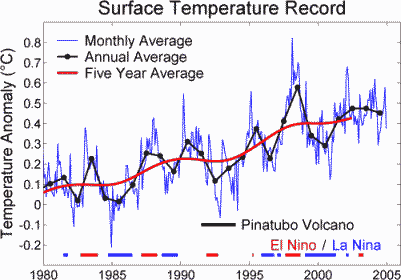
\includegraphics{images/image054.png}
\caption{Image prepared by Robert A. Rohde,
\url{http://commons.wikimedia.org/wiki/File:Short_Instrumental_Temperature_Record.png}.}
\end{figure}

Typically the average function reveals the pattern much more clearly
than the original data. This use of a ``moving average'' value of
``noisy'' data (weather information, stock prices) is a very common.

To view this video please enable JavaScript, and consider upgrading to a
web browser that \href{http://videojs.com/html5-video-support/}{supports
HTML5 video}

\hypertarget{example-2}{%
\paragraph{Example 2}\label{example-2}}

The graph below shows the amount of water in a reservoir over a 12 hour
period. Estimate the average amount of water in the reservoir over this
period.

\begin{figure}
\centering
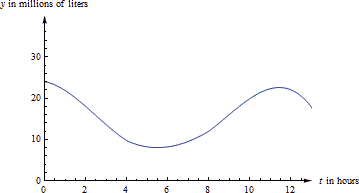
\includegraphics{images/image055.png}
\caption{}
\end{figure}

If \textbackslash{}( V(t) \textbackslash{}) is the volume of the water
(in millions of liters) after \textbackslash{}(t\textbackslash{}) hours,
then the average amount is \textbackslash{}(
\textbackslash{}frac\{1\}\{12\}\textbackslash{},\textbackslash{}int\_0\^{}\{12\}
V(t)\textbackslash{}, dt \textbackslash{}). In order to find the
definite integral, we'll have to estimate. Let's use 6 rectangles and
take the heights from their right edges (there's nothing special about
using 6 rectangles or right edges -- other choices would still give you
a valid estimate).

\begin{figure}
\centering
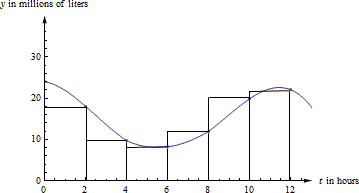
\includegraphics{images/image056.png}
\caption{}
\end{figure}

The estimate of the integral is
\textbackslash{}{[}\textbackslash{}int\_0\^{}\{12\}
V(t)\textbackslash{}, dt \textbackslash{}approx
(18)(2)+(9.7)(2)+(8.2)(2)+(12)(2)+(19.9)(2)+(22)(2)=179.6.\textbackslash{}{]}

The units of this integral are (millions of liters)\textbackslash{}(
\textbackslash{}cdot \textbackslash{})(feet). So our estimate of the
average volume is \textbackslash{}(
\textbackslash{}frac\{1\}\{12\}\textbackslash{}cdot
179.6\textbackslash{}approx 15 \textbackslash{}) millions of liters.
(The estimate might change a little depending on how we estimate the
function values from the graph.)

In the figure below, you can see the same graph with the line
\textbackslash{}( y=15 \textbackslash{}) drawn in. The area under the
curve and the area under the rectangle are (approximately) the same.

\begin{figure}
\centering
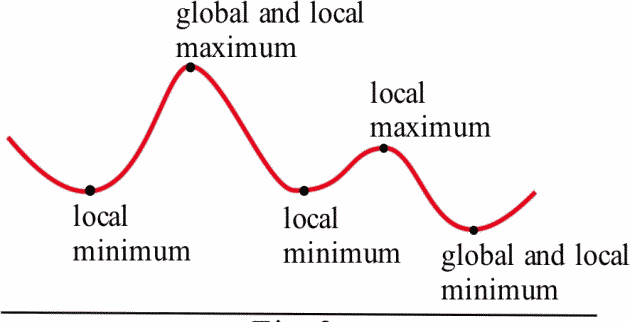
\includegraphics{images/image057.png}
\caption{}
\end{figure}

In fact, that would be a different way to estimate the average value. We
could have estimated the placement of the horizontal line so that the
area under the curve and under the line were equal.

\hypertarget{area}{%
\subsection{Area}\label{area}}

We have already used integrals to find the area between the graph of a
function and the horizontal axis. Integrals can also be used to find the
area between two graphs.

If \textbackslash{}(f(x) \textbackslash{}geq g(x)\textbackslash{}) for
all \textbackslash{}(x\textbackslash{}) in
\textbackslash{}({[}a,b{]}\textbackslash{}), then we can approximate the
area between \textbackslash{}(f\textbackslash{}) and
\textbackslash{}(g\textbackslash{}) by partitioning the interval
\textbackslash{}({[}a,b{]}\textbackslash{}) and forming a Riemann sum,
as shown in the picture. The height of each rectangle is top - bottom,
\textbackslash{}(f(c\_i) - g(c\_i)\textbackslash{}) so the area of the
\textbackslash{}(i\textbackslash{})-th rectangle is
(height)\textbackslash{}( \textbackslash{}cdot \textbackslash{})(base) =
\textbackslash{}(\textbackslash{}left(f(c\_i) -
g(c\_i)\textbackslash{}right)\textbackslash{}cdot\textbackslash{}Delta
x\textbackslash{}). Adding up these rectangles gives an approximation of
the total area as \textbackslash{}( \textbackslash{}sum\_\{i=1\}\^{}n
\textbackslash{}left(f(c\_i) -
g(c\_i)\textbackslash{}right)\textbackslash{}cdot\textbackslash{}Delta x
\textbackslash{}), a Riemann sum.

\begin{figure}
\centering
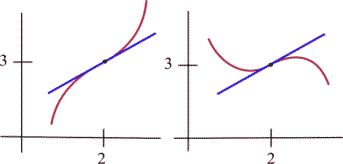
\includegraphics{images/image049.png}
\caption{}
\end{figure}

The limit of this Riemann sum, as the number of rectangles gets larger
and their width gets smaller, is the definite integral \textbackslash{}(
\textbackslash{}int\_a\^{}b \textbackslash{}left(f(c\_i) -
g(c\_i)\textbackslash{}right)\textbackslash{}, dx \textbackslash{}).

To view this video please enable JavaScript, and consider upgrading to a
web browser that \href{http://videojs.com/html5-video-support/}{supports
HTML5 video}

\hypertarget{area-between-two-curves}{%
\paragraph{Area Between Two Curves}\label{area-between-two-curves}}

The area between two curves \textbackslash{}(f(x)\textbackslash{}) and
\textbackslash{}(g(x)\textbackslash{}), where \textbackslash{}(f(x)
\textbackslash{}geq g(x)\textbackslash{}), between \textbackslash{}(x =
a\textbackslash{}) and \textbackslash{}(x = b\textbackslash{}) is
\textbackslash{}{[} \textbackslash{}int\_a\^{}b
\textbackslash{}left(f(c\_i) -
g(c\_i)\textbackslash{}right)\textbackslash{}, dx. \textbackslash{}{]}

The integrand is ``top - bottom.'' Make a graph or use test values to be
sure which curve is which.

\hypertarget{example-3}{%
\paragraph{Example 3}\label{example-3}}

Find the area bounded between the graphs of \textbackslash{}(f(x) =
x\textbackslash{}) and \textbackslash{}(g(x) = 3\textbackslash{}) for
\textbackslash{}(1 \textbackslash{}leq x \textbackslash{}leq
4\textbackslash{}).

\begin{figure}
\centering
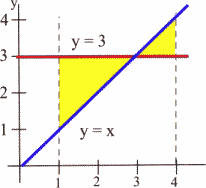
\includegraphics{images/image050.png}
\caption{}
\end{figure}

Always start with a graph so you can see which graph is the top and
which is the bottom. In this example, the two curves cross, and they
change positions; we'll need to split the area into two pieces.
Geometrically, we can see that the area is 2 + 0.5 = 2.5.

Writing the area as a sum of definite integrals, we get
\textbackslash{}{[} \textbackslash{}text\{Area \}=
\textbackslash{}int\_1\^{}3 (3-x)\textbackslash{},
dx+\textbackslash{}int\_3\^{}4 (x-3)\textbackslash{},
dx.\textbackslash{}{]}

These integrals are easy to evaluate using antiderivatives:
\textbackslash{}{[} \textbackslash{}begin\{align*\}
\textbackslash{}int\_1\^{}3 (3-x)\textbackslash{}, dx=\&
\textbackslash{}left{[}3x-\textbackslash{}frac\{x\^{}2\}\{2\}\textbackslash{}right{]}\_1\^{}3
\textbackslash{}\textbackslash{} =\&
\textbackslash{}left(9-\textbackslash{}frac\{9\}\{2\}\textbackslash{}right)-\textbackslash{}left(15-\textbackslash{}frac\{25\}\{2\}\textbackslash{}right)
\textbackslash{}\textbackslash{} =\& 2 \textbackslash{}end\{align*\}
\textbackslash{}{]} \textbackslash{}{[} \textbackslash{}begin\{align*\}
\textbackslash{}int\_3\^{}4 (x-3)\textbackslash{}, dx=\&
\textbackslash{}left{[}\textbackslash{}frac\{x\^{}2\}\{2\}-3x\textbackslash{}right{]}\_3\^{}4
\textbackslash{}\textbackslash{} =\&
\textbackslash{}left(\textbackslash{}frac\{16\}\{2\}-12\textbackslash{}right)-\textbackslash{}left(\textbackslash{}frac\{9\}\{2\}-9\textbackslash{}right)
\textbackslash{}\textbackslash{} =\& \textbackslash{}frac\{1\}\{2\}
\textbackslash{}end\{align*\} \textbackslash{}{]}

The sum of these two integrals tells us that the total area between
\textbackslash{}(f\textbackslash{}) and
\textbackslash{}(g\textbackslash{}) is 2.5 square units, which we
already knew from the picture.

Note that the single integral \textbackslash{}(
\textbackslash{}int\_1\^{}4 (3-x)\textbackslash{}, dx = 1.5
\textbackslash{}) is not the \textbf{area} we want in the last example.
The value of \textbf{the integral is 1.5}, and the value of \textbf{the
area is 2.5}. That's because for the triangle on the right, the graph of
\textbackslash{}(y = x\textbackslash{}) is above the graph of
\textbackslash{}(y = 3\textbackslash{}), so the integrand
\textbackslash{}(3 - x\textbackslash{}) is negative; in the definite
integral, the area of that triangle comes in with a negative sign.

In this example, it was easy to see exactly where the two curves crossed
so we could break the region into the two pieces to figure separately.
In other examples, you might need to solve an equation to find where the
curves cross.

To view this video please enable JavaScript, and consider upgrading to a
web browser that \href{http://videojs.com/html5-video-support/}{supports
HTML5 video}

\hypertarget{example-4}{%
\paragraph{Example 4}\label{example-4}}

Two objects start from the same location and travel along the same path
with velocities \textbackslash{}( v\_A(t)=t+3 \textbackslash{}) and
\textbackslash{}( v\_B(t)=t\^{}2-4t+3 \textbackslash{}) meters per
second. How far ahead is \textbackslash{}(A\textbackslash{}) after 3
seconds?

\begin{figure}
\centering
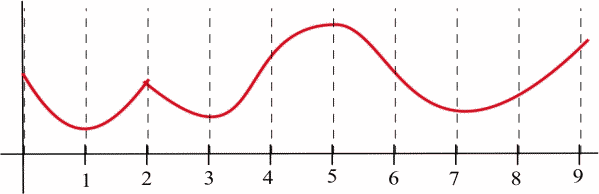
\includegraphics{images/image051.png}
\caption{}
\end{figure}

Since \textbackslash{}( v\_A(t) \textbackslash{}geq v\_B(t)
\textbackslash{}) , the ``area'' between the graphs of \textbackslash{}(
v\_A \textbackslash{}) and \textbackslash{}( v\_B \textbackslash{})
represents the distance between the objects.

After 3 seconds, the distance apart is \textbackslash{}{[}
\textbackslash{}begin\{align*\} \textbackslash{}int\_0\^{}3
\textbackslash{}left( v\_A(t) - v\_B(t)
\textbackslash{}right)\textbackslash{}, dt=\&
\textbackslash{}int\_0\^{}3 \textbackslash{}left( (t+3) -
\textbackslash{}left( t\^{}2-4t+3 \textbackslash{}right)
\textbackslash{}right)\textbackslash{}, dt
\textbackslash{}\textbackslash{} =\& \textbackslash{}int\_0\^{}3
\textbackslash{}left(5t-t\^{}2\textbackslash{}right)\textbackslash{}, dt
\textbackslash{}\textbackslash{} =\& \textbackslash{}left{[}
5\textbackslash{}frac\{t\^{}2\}\{2\}
-\textbackslash{}frac\{t\^{}3\}\{3\} \textbackslash{}right{]}\_0\^{}3
\textbackslash{}\textbackslash{} =\& \textbackslash{}left(
5\textbackslash{}frac\{9\}\{2\}-\textbackslash{}frac\{27\}\{3\}\textbackslash{}right)-(0)
\textbackslash{}\textbackslash{} =\& 13.5 \textbackslash{}text\{
meters\}. \textbackslash{}end\{align*\} \textbackslash{}{]}

To view this video please enable JavaScript, and consider upgrading to a
web browser that \href{http://videojs.com/html5-video-support/}{supports
HTML5 video}

\hypertarget{volume}{%
\subsection{Volume}\label{volume}}

Just as we can partition an interval and imagine approximating an area
with rectangles to find a formula for the area between curves, we can
partition an interval and imagine approximating a volume with simple
shapes to find a formula for the volume of a solid. While this approach
works for a variety of shapes, our focus will be on shapes formed by
revolving a curve around the horizontal axis.

We start with an area, the region below a function on the interval
\textbackslash{}(a \textbackslash{}leq x \textbackslash{}leq
b\textbackslash{}). We are going to take that region, and rotate it
around the \textbackslash{}(x\textbackslash{})-axis, creating the solid
shape shown.

\begin{figure}
\centering
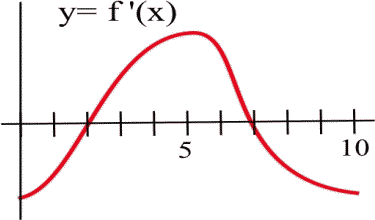
\includegraphics{images/image070.png}
\caption{}
\end{figure}

To find the volume of this solid, we can start by partitioning the
interval {[}0,1{]} and approximating the area with rectangles. As
before, the width of each rectangle would be \textbackslash{}(
\textbackslash{}Delta x \textbackslash{}) and the height
\textbackslash{}(f(c\_i)\textbackslash{}).

\begin{figure}
\centering
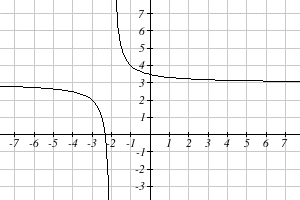
\includegraphics{images/image071.png}
\caption{}
\end{figure}

If we took just one of these rectangles and rotated it about the
horizontal axis, it would form a cylindrical shape. The radius of that
cylinder would be \textbackslash{}(f(c\_i)\textbackslash{}), so the
volume would be \textbackslash{}{[} V=\textbackslash{}pi r\^{}2
h=\textbackslash{}pi\textbackslash{}left(f(c\_i)\textbackslash{}right)\^{}2\textbackslash{}Delta
x. \textbackslash{}{]}

The volume of the whole solid could be approximated by rotating each of
the rectangles about the x axis. Adding up the volume of each of the
little cylindrical discs gives an approximation of the total volume as
\textbackslash{}(
\textbackslash{}sum\textbackslash{}limits\_\{i=1\}\^{}n
\textbackslash{}pi\textbackslash{}left(f(c\_i)\textbackslash{}right)\^{}2\textbackslash{}Delta
x \textbackslash{}), a Riemann sum.

The limit of this sum as the width of the rectanges becomes small is the
definite integral \textbackslash{}( \textbackslash{}int\_a\^{}b
\textbackslash{}pi\textbackslash{}left(f(c\_i)\textbackslash{}right)\^{}2\textbackslash{},
dx \textbackslash{})

\hypertarget{volume-1}{%
\paragraph{Volume}\label{volume-1}}

The volume of the solid obtained by rotating about the
\textbackslash{}(x\textbackslash{})-axis the area bounded by the curve
\textbackslash{}(f(x)\textbackslash{}), the
\textbackslash{}(x\textbackslash{})-axis, \textbackslash{}(x =
a\textbackslash{}), and \textbackslash{}(x = b\textbackslash{}) is
\textbackslash{}{[} \textbackslash{}int\_a\^{}b
\textbackslash{}pi\textbackslash{}left(f(c\_i)\textbackslash{}right)\^{}2\textbackslash{},
dx \textbackslash{}{]}

\hypertarget{example-5}{%
\paragraph{Example 5}\label{example-5}}

Find the volume of the solid formed by rotating the area under
\textbackslash{}( f(x)=e\^{}\{-x\} \textbackslash{}) on the interval
{[}0,1{]} about the \textbackslash{}(x\textbackslash{})-axis.

\begin{figure}
\centering
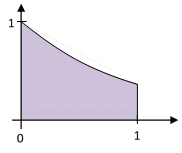
\includegraphics{images/image073.png}
\caption{}
\end{figure}

This is the region pictured in the earlier example. We substitute in the
function and bounds into the formula we derived to set up the definite
integral: \textbackslash{}{[} \textbackslash{}text\{Volume\} =
\textbackslash{}int\_0\^{}1
\textbackslash{}pi\textbackslash{}left(e\^{}\{-x\}\textbackslash{}right)\^{}2\textbackslash{},
dx. \textbackslash{}{]}

Using exponent rules, the integrand can be simplified. The constant
\textbackslash{}( \textbackslash{}pi \textbackslash{}) can be pulled out
of the integral: \textbackslash{}{[} \textbackslash{}text\{Volume\} =
\textbackslash{}pi\textbackslash{}int\_0\^{}1
e\^{}\{-2x\}\textbackslash{}, dx. \textbackslash{}{]}

Using the substitution \textbackslash{}(u = -2x\textbackslash{}), we can
integrate this function. \textbackslash{}{[}
\textbackslash{}begin\{align*\}
\textbackslash{}pi\textbackslash{}int\_0\^{}1
e\^{}\{-2x\}\textbackslash{}, dx=\&
\textbackslash{}text\{(\textbackslash{}( u
\textbackslash{})-substitution)\} \textbackslash{}\textbackslash{} =\&
\textbackslash{}left. -\textbackslash{}frac\{1\}\{2\}\textbackslash{}pi
e\^{}\{-2x\}\textbackslash{}right{]}\_0\^{}1
\textbackslash{}\textbackslash{} =\&
\textbackslash{}left(-\textbackslash{}frac\{1\}\{2\}\textbackslash{}pi
e\^{}\{-2(1)\}\textbackslash{}right) -
\textbackslash{}left(-\textbackslash{}frac\{1\}\{2\}\textbackslash{}pi
e\^{}\{-2(0)\}\textbackslash{}right) \textbackslash{}\textbackslash{}
\textbackslash{}approx \& 1.358\textbackslash{}text\{ cubic units\}.
\textbackslash{}end\{align*\} \textbackslash{}{]}

\begin{longtable}[]{@{}ll@{}}
\toprule
\endhead
\href{section3-5.php}{← Previous Section} & \href{section3-7.php}{Next
Section →}\tabularnewline
\bottomrule
\end{longtable}
